% !TEX root = ../document.tex

\chapter{\label{ch:spoofax}Background: The Spoofax language workbench}

Before discussing what properties a language like Dynamix may need, we first need to discuss the context in which it will be used. Dynamix was designed to be used within the Spoofax language workbench \cite{Spoofax2021}, a software suite that combines various meta-languages and tools that allow a user to easily design and implement (domain-specific) programming languages. Within Spoofax, the Dynamix meta-language needs to be able to interact with the results of other languages and analyses, such as the parsed \ac{AST} and the results of any static analysis.

This chapter introduces several parts of the Spoofax language workbench that are relevant for understanding the design choices and context in which Dynamix will be used. In particular, we discuss the \ac{AST} representation that Spoofax uses, how it performs static analysis, and the conventions that Spoofax meta-languages follow. Carefully considering these aspects will ensure that Dynamix feels a natural addition to the Spoofax language workbench and that users familiar with other Spoofax meta-languages can easily start working with Dynamix.

\todo[inline]{either extend this introduction or introduce a new section first that gives a brief overview of the Spoofax organization, list of meta-languages, Eclipse, Spoofax 3, etc}

\section{\label{sec:spoofax_parsing_aterm}Syntax definition and parsing}

The natural first part of a language workbench is the ability to declare a grammar for the language. For this purpose, Spoofax offers the Syntax Definition Formalism 3 (SDF3) meta-language \cite{Amorim2019}. Using SDF3, a user is able to declare both lexical and context-free syntax productions for their language. From this declaration, SDF3 generates a scannerless parser with support for error recovery, a pretty-printer and a syntax highlighter \cite{AmorimV20}.\\

\Cref{fig:sdf3_example} shows an example of an SDF3 definition for a simple arithmetic language. Two lexical sorts are defined, \texttt{INT} and \texttt{ID} which represent an integer literal and variable identifier respectively. A single context-free sort is defined, \texttt{Exp}, which represent an arbitrary expression. Here, the difference between a lexical and a context-free production determines whether implicit layout such as spaces is allowed between subterms of the production and affects the parsing output of the production (a lexical production yields a string of its contents, whereas a context-free production produces a tuple containing its subterms).\\

The \texttt{LAYOUT} syntax-production in line 7\todo{check/fix line numbers} is used to allow implicit layout between terms in context-free productions. Without this declaration, an expression such as \texttt{1 + 2} would be rejected as invalid. This may be surprising since the syntax for addition is defined with explicit spaces surrounding the \texttt{+} token. Indeed, SDF3 treats this declaration as \texttt{Exp LAYOUT? '+' LAYOUT? Exp}, and only uses the formatting supplied by the language author for the generated pretty-printer.\\

The grammar in \cref{fig:sdf3_example} is ambiguous: the expression \texttt{1 + 2 * 3} can be parsed as either \texttt{(1 + 2) * 3} or \texttt{1 + (2 * 3)}. This is resolved through the use of the \textbf{\texttt{context-free priorities}} section (line 25-26). Here, we explicitly state that the division and multiplication operators should bind more tightly than the addition and subtraction operators. Within the same precedence level, each operator is marked as left-associative by annotating its group with \texttt{left:}. The \texttt{\{bracket\}} production in line 15 allows for brackets to be used to explicitly enforce order of operations. The pretty-printer generated by SDF3 will only include these brackets in the output if they are necessary.\\

\begin{figure}
  \begin{sdf3}
module start

lexical sorts INT ID
lexical syntax
  INT = [1-9] [0-9]*
  ID = [A-Za-z] [A-Za-z0-9]*
  LAYOUT = [\ \n\r\t]

context-free sorts Exp
context-free syntax
  Exp = <(<Exp>)> {bracket}
  Exp.Add = <<Exp> + <Exp>> {left}
  Exp.Sub = <<Exp> - <Exp>> {left}
  Exp.Mul = <<Exp> * <Exp>> {left}
  Exp.Div = <<Exp> / <Exp>> {left}

  Exp.Var = <<ID>>
  Exp.Int = <<INT>>

  Exp.Let = <let <ID> = <Exp> in <Exp>>

context-free priorities
  {left: Exp.Mul Exp.Div} > {left: Exp.Add Exp.Sub} > {Exp.Let}
  \end{sdf3}
  \caption{A simple SDF3 grammar for an arithmetic language that supports variable bindings.}
  \label{fig:sdf3_example}
\end{figure}

\todo{reorder aterm grammar and example output?}
The parser generated by SDF3 ouputs an \ac{AST} in the \acf{ATerm}. This format originated in the ASF+SDF formalism \cite{DHP:1996}, a precursor to the Spoofax language workbench. It is a simple data transfer format that supports strings, integers, lists, tuples, tagged tuples (constructors), and annotations. The grammar for the ATerm format can be seen in \cref{fig:aterm_grammar}. \acp{ATerm} are used pervasively across the Spoofax language workbench and are supported as data format in all Spoofax meta-languages. \Cref{fig:sdf3_example_parse_output} shows an example of the parsing output for a simple program using the grammar defined in \cref{fig:sdf3_example}.\\

\todo{string char grammar? right now it is not explicitly defined}

\begin{figure}
  \begin{lstlisting}
<term> ::= <int literal>
  | <string literal>
  | <identifier> '(' <terms> ')'
  | '[' <terms> ']'
  | '(' <terms> ')'
  | <term> '{' <terms> '}'

<int literal> ::= [1-9] [0-9]*
<string literal> ::= '"' <string char*> '"'
<identifier> ::= [A-Za-z] [A-Za-z0-9._-]*
<terms> ::=
  | <term>
  | <term> ',' <terms>
  \end{lstlisting}
  \caption{The grammar for the \ac{ATerm} data representation format.}
  \label{fig:aterm_grammar}
\end{figure}

\begin{figure}
  \centering
  \begin{subfigure}{.35\textwidth}
    \centering
    \begin{mat}
let x = 10 in
  let y = 20 in
    let z = x + y in
      (10 + x) * y / z
    \end{mat}
  \end{subfigure}\hfill%
  \begin{subfigure}{.585\textwidth}
    \centering
    \begin{statix*}{firstline=5,lastline=20,firstnumber=1}
module main

rules
  foo(
Let(
  "x",
  Int("10"),
  Let(
    "y",
    Int("20"),
    Let(
      "z",
      Add(Var("x"), Var("y")),
      Div(
        Mul(Add(Int("10"), Var("x")), Var("y")),
        Var("z")
      )
    )
  )
)
  ).
    \end{statix*}
  \end{subfigure}
  \caption{An example expression in the arithmetic language declared in \cref{fig:sdf3_example}\protect\footnotemark. The parsed \ac{AST} in \ac{ATerm} format as produced by the generated parser can be seen on the right.}
  \label{fig:sdf3_example_parse_output}
\end{figure}

\todo{ensure footnote on correct page}
\footnotetext{The syntax highlighting in this snippet is exactly the syntax highlighting that SDF3 automatically generates using the grammar definition.}

From the SDF3 declaration we can also deduce an \textit{algebraic signature}. Such a signature dictates the exact structure that an \ac{ATerm} expression can take such that it is a valid AST\footnote{Here, valid \ac{AST} means that it is an \ac{AST} that can be produced by the parser (i.e. it has a lexical equivalent), and not necessarily that this \ac{AST} is valid according to the static and dynamic semantics of the language.}. These signatures are automatically generated by SDF3 and are used by various other meta-languages in the Spoofax language workbench to provide static-analysis features. \Cref{fig:sdf3_example_signature} shows the signature for the example grammar in both formal and Spoofax syntax formats.\\

% For some reason this "centers" the algebraic signature and the statix signature.
\newsavebox{\sdfsignaturebox}
\begin{lrbox}{\sdfsignaturebox}\begin{minipage}{.45\textwidth}
\begin{statix*}{firstline=3,firstnumber=1}
module main

signature
  sorts
    INT = string
    ID = string
    Exp

  constructors
    Add : Exp * Exp -> Exp
    Sub : Exp * Exp -> Exp
    Mul : Exp * Exp -> Exp
    Div : Exp * Exp -> Exp
    Var : ID -> Exp
    Int : INT -> Exp
    Let : ID * Exp * Exp -> Exp
\end{statix*}
\end{minipage}
\end{lrbox}

\begin{figure}
  \centering
  \begin{subfigure}{.45\textwidth}
    \centering
    \usebox{\sdfsignaturebox}
  \end{subfigure}\hfill%
  \begin{subfigure}{.5\textwidth}
    \centering
    $$ S = \{\texttt{INT}, \texttt{ID}, \texttt{Exp}\} $$
    \begin{equation*}
    \begin{aligned}
    \Sigma = \{ \; & \texttt{Add} : \texttt{Exp} \times \texttt{Exp} \to \texttt{Exp}, \\
                  & \texttt{Sub} : \texttt{Exp} \times \texttt{Exp} \to \texttt{Exp}, \\
                  & \texttt{Mul} : \texttt{Exp} \times \texttt{Exp} \to \texttt{Exp}, \\
                  & \texttt{Div} : \texttt{Exp} \times \texttt{Exp} \to \texttt{Exp}, \\
                  & \texttt{Var} : \texttt{ID} \to \texttt{Exp}, \\
                  & \texttt{Int} : \texttt{INT} \to \texttt{Exp}, \\
                  & \texttt{Let} : \texttt{ID} \times \texttt{Exp} \times \texttt{Exp} \to \texttt{Exp} \; \}
    \end{aligned}
    \end{equation*}
  \end{subfigure}
  \caption{The algebraic signature for the grammar in \Cref{fig:sdf3_example}. Left shows the signature of the grammar defined in the Statix meta-language, right shows the grammar in equivalent formal term algebra notation. The left source is automatically derived from the grammar definition by SDF3 as part of the compilation process.}
  \label{fig:sdf3_example_signature}
\end{figure}

Other features that SDF3 offers include the ability to specify layout constraints for grammar productions (often crucial for languages that have significant whitespace such as Python and Haskell), bla bla bla\todo{properly end this section, also less/good cites?}. For more information on SDF3 and parsing within the Spoofax language workbench, the reader is invited to consult \cite{KatsV10a, Spoofax2021, Amorim2019, AmorimV20,KallebergV07, WachsmuthKV14}.

\section{\label{sec:spoofax_constraint}Static analysis with constraint solvers}

Now, we briefly discuss the approach Spoofax takes with regards to static analysis. It is important to discuss this property, since the exact runtime semantics of an expression in a language may be determined by aspects such as the types involved in the expression (e.g. the additive operator is often overloaded for both integers and strings). Any \ac{DSL} designed for use within the Spoofax ecosystem will therefore almost certainly need a way to interact with the results of the static analysis.\\

\todo{more info on statix? really shallow right now, but we don't use it much outside of properties}
The current meta-language used for static analysis in the Spoofax workbench is Statix \cite{AntwerpenPRV18}. Statix is a declarative language that performs static analysis through the use of constraints. A Statix specification consists of a set of declarative rules that specify constraints that should hold for a program to be valid. If the Statix logic solver can find a solution for which all constraints hold for a given input \ac{AST}, a program is considered well-typed. Name binding correctness is asserted through the use of \textit{scope graphs} \cite{TUD-SERG-2015-009}, although their exact semantics are beyond the scope of this paper. The reader is referred to the work by van Antwerpen et al. \cite{TUD-SERG-2015-009,AntwerpenPRV18,VanAntwerpen2016} should they be interested in their exact workings. \\

\Cref{fig:stx_example} shows an example typing rule in both formal notation and Statix syntax. The \texttt{typeOfExpression} rule and $\Gamma \vdash v : \texttt{T}$ notation are equivalent, in that they both describe the relationship between an expression and its type. Within the \textit{head} of the Statix rule, the \texttt{Div(a, b)} node is pattern-matching on exactly the \ac{ATerm} that is output by the parser. Indeed, all values in Statix (including the \texttt{INT()} term) are \acp{ATerm}. Using the signatures generated by SDF3 (see \cref{sec:spoofax_parsing_aterm}, \cref{fig:sdf3_example_signature}), the Statix meta-language can statically ensure that these pattern-matching operations are valid.\\

Beyond simply indicating whether some input \ac{AST} is valid according to the Statix specification, the Statix solver also allows users to attach \textit{properties} to arbitary AST nodes. These properties are arbitrary \ac{ATerm} values and can later be read from outside Statix. Common properties used in Statix specifications are the \texttt{ref} and \texttt{type} properties, which represent the declaring node and the type of a node respectively. The Spoofax language workbench has built-in support for reading the values of these two properties to provide editor services such as hover hints and go-to-definition. An example of the \texttt{type} annotation, as well as the tooltip generated as a result, can be seen in \cref{fig:stx_property_example}. It is worth pointing out that both the \texttt{type} and \texttt{ref} properties are simply conventions. A user is able to assign arbitrary properties to a property, and can read these values from other meta-languages within the Spoofax language workbench.

\begin{figure}
  \centering
  \begin{subfigure}{.55\textwidth}
    \centering
    \begin{statix*}{firstline=3,firstnumber=1}
module main

rules
  typeOfExpression(s, Div(a, b)) = INT() :-
    typeOfExpression(s, a) == INT(),
    typeOfExpression(s, b) == INT().
    \end{statix*}
  \end{subfigure}\hfill%
  \begin{subfigure}{.45\textwidth}
    \centering
    \begin{prooftree}
    \AxiomC{$\Gamma \vdash a : \texttt{INT}$}
    \noLine
    \UnaryInfC{$\Gamma \vdash b : \texttt{INT}$}
    \RightLabel{T-Division}
    \UnaryInfC{$\Gamma \vdash a \mathbin{/} b : \texttt{INT}$}
    \end{prooftree}
  \end{subfigure}
  \caption{An example typing rule for integer division in both Statix notation and formal notation. Here \texttt{s} and $\Gamma$ are analogous and correspond to the context in which the expression appears. Other rules, such as the type of an integer literal, are omitted.}
  \label{fig:stx_example}
\end{figure}

\begin{figure}
  \centering
  \begin{subfigure}{.55\textwidth}
    \centering
    \begin{statix*}{firstline=3,firstnumber=1,highlightlines={5}}
module main

rules
  typeOfExpression(s, n@Div(a, b)) = INT() :-
    typeOfExpression(s, a) == INT(),
    typeOfExpression(s, b) == INT(),
    @n.type := INT().
    \end{statix*}
  \end{subfigure}\hfill%
  \begin{subfigure}{.40\textwidth}
    \centering
    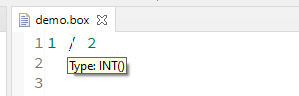
\includegraphics{img/stx_hover_example.png}
  \end{subfigure}
  \caption{An example showing the ability to attach properties to nodes in Statix. The highlighted line (left) sets the \texttt{type} property on the AST node representing the division expression. This value is later read by Spoofax to provide editor services such as hover information (right).}
  \label{fig:stx_property_example}
\end{figure}

\section{\label{sec:spoofax_transform}Transformations using Stratego}

section needed? stratego isn't really used besides implementing the interpreter inside them? depends on whether we discuss the interpreter at all? is it worth it to explain the entirety of stratego here for some extra background information? we will likely discuss (mini-)stratego as part of the case study anyway
\todo{see text}